% !TEX root = ../my-thesis.tex
%
\chapter{Appendix}
\label{sec:appendix}
\section{Probability Distributions and the Exponential Family}
\subsection{The Exponential Family}
In statistics and probability theory, the \textit{exponential family} is a parametric set of probability distributions of a specific form. The distribution of a random variable $\pmb{y}$ belongs to the exponential family if the discrete or continuous density with respect to a $\sigma$-finite measure of $\pmb{y}$ has the form
\begin{equation}
    f(\pmb{y}|\pmb{\theta}, \lambda)=\exp\left(\frac{\pmb{y}^T\pmb{\theta} - b(\pmb{\theta})}{\lambda}+c(\pmb{y},\lambda) \right),
\end{equation}
with $c(\pmb{y},\lambda)\geq 0$. 
$\pmb{\theta}\in\Theta\subset\mathbb{R}^q$ is the \textit{natural} or \textit{canonical} parameter of the exponential family, while $\lambda > 0$ is a \textit{dispersion} or \textit{nuisance} parameter \autocite[][]{holland1981exponential}. The natural parameter space $\Theta$ is the set of all $\pmb{\theta}$ satisfying
\begin{equation}
    0<\int\exp\left(\left(\pmb{y}^T\pmb{\theta} - b(\pmb{\theta})\right)/\lambda+c(\pmb{y},\lambda) \right)d\pmb{y}< \infty
\end{equation} Moreover, $b(\pmb{\theta})$ is a twice differentiable  function and all moments of $\pmb{y}$ exist. Specifically, 
\begin{alignat}{3}
    \mathbb{E}_{\pmb{\theta}}(\pmb{y}) &= \mu(\pmb{\theta}) =& \frac{\partial b(\pmb{\theta})}{\partial\pmb{\theta}} \\
    \hbox{Cov}_{\pmb{\theta}}(\pmb{y}) &= \pmb{\Sigma}(\pmb{\theta}) =& \lambda\frac{\partial^2b(\pmb{\theta})}{\partial\pmb{\theta}\partial\pmb{\theta}^T}.
\end{alignat}
The covariance matrix $\pmb{\Sigma}(\pmb{\theta})$ is positive definite in $\Theta^0$, therefore $\mu:\Theta^0\rightarrow  M = \mu\left(\Theta^0\right)$ is injective. By substituting the inverse function $\pmb{\theta}(\mu)$ into $\frac{\partial^2b(\pmb{\theta})}{\partial\pmb{\theta}\partial\pmb{\theta}^T}$, the variance function 
\begin{equation}
    v(\mu)=\frac{\partial^2b(\pmb{\theta}(\mu))}{\partial\pmb{\theta}\partial\pmb{\theta}^T}
\end{equation}
is given and the covariance can be written as
\begin{equation}
    \hbox{Cov}_{\pmb{\theta}}(\pmb{y}) = \lambda v(\mu).
\end{equation}
Important members of the exponential family are the normal, binomial, Poisson, gamma and multivariate normal distribution \autocite[][433]{fahrmeir2013multivariate}.
\subsection{The Normal Distribution}
The normal distribution is an important type of continuous probability distribution in stochastics. The special significance of the normal distribution is based, among other things, on the central limit theorem, according to which distributions that result from the additive combination of a large number of independent influences are approximately normally distributed under weak conditions. \\
The density is given by
\begin{equation}
    f\left(\pmb{x}|\mu,\sigma\right)=\frac{1}{\sigma\sqrt{2\pi}}\exp\left(-\frac{1}{2}\left(\frac{\pmb{x}-\mu}{\sigma}\right)^2\right).
\end{equation}
The first two moments of the distribution are given by
\begin{align}
    \mathbb{E}\left[X\right] &= \mu \\
    \hbox{Var}\left[X\right] &= \sigma^2.
\end{align}
The graph of this density function has a "bell-shaped form" and is symmetrical with $\mu$ as the centre of symmetry \autocite[][83-85]{fahrmeir2016statistik}.
\subsection{The Multivariate Normal Distribution}
The density of a normally distributed random variable $\pmb{y}=\left(y_1,...,y_n\right)^T, n<\infty$ with mean vector $\pmb{\mu}$ ($n\times1$) and SPD covariance matrix $\pmb{\Sigma}$ ($n\times n$) is
\begin{equation}
    \pi\left(\pmb{y}\right)=\left(2\pi\right)^{-n/2}|\pmb{\Sigma}|^{-1/2}\exp\left(-\frac{1}{2}\left(\pmb{y}-\pmb{\mu}\right)^T\pmb{\Sigma}^{-1}\left(\pmb{y}-\pmb{\mu}\right)\right),\hspace{5pt}\pmb{y}\in\mathbb{R}^n
\end{equation}
Here, $\mu_i=\mathbb{E}\left[y_i\right]$, $ \Sigma_{ij}=\hbox{Cov}\left(y_i,y_j\right)$, $ \Sigma_{ii}=\hbox{Var}\left(y_i\right) > 0$ and $\hbox{Corr}\left(y_i,y_j\right)=\Sigma_{ij}/\left(\Sigma_{ii}\Sigma_{jj}\right)^{1/2}$. This is written as $\pmb{y}\sim\mathcal{N}\left(\pmb{\mu},\pmb{\Sigma}\right)$. For $n=1$, $\mu=0$ and $\Sigma_{11}=1$ the standard normal distribution is obtained. \\
$\pmb{y}$ is now split up into $\pmb{y}=\left(\pmb{y}_{\pmb{A}}^T,\pmb{y}_{\pmb{B}}^T\right)$ and $\pmb{\mu}$ and $\pmb{\Sigma}$ are divided accordingly:
\begin{equation*}
    \pmb{\mu} = \begin{pmatrix}\pmb{\mu}_{\pmb{A}} \\ \pmb{\mu}_{\pmb{B}}\end{pmatrix} \hspace{20pt}\hbox{ and }\hspace{20pt} \pmb{\Sigma}=\begin{pmatrix}\pmb{\Sigma}_{\pmb{AA}} & \pmb{\Sigma}_{\pmb{AB}}\\\pmb{\Sigma}_{\pmb{BA}} & \pmb{\Sigma}_{\pmb{BB}}\end{pmatrix}.
\end{equation*}
Some basic properties of the multivariate normal distribution are the following.
\begin{itemize}
    \item[1.] $\pmb{y}_{\pmb{A}}\sim\mathcal{N}\left(\pmb{\mu}_{\pmb{A}}, \pmb{\Sigma}_{\pmb{AA}}\right)$.
    \item[2.] $\pmb{\Sigma}_{\pmb{AB}}=\pmb{0}$ precisely when $\pmb{y}_{\pmb{A}}$ and $\pmb{y}_{\pmb{B}}$ are independent.
    \item[3.] The conditional distribution $\pi\left(\pmb{y}_{\pmb{A}}|\pmb{y}_{\pmb{B}}\right)$ is $\mathcal{N}\left(\pmb{\mu}_{\pmb{A}|\pmb{B}}, \pmb{\Sigma}_{\pmb{A}|\pmb{B}}\right)$, where
    \begin{align*}
        \pmb{\mu}_{\pmb{A}|\pmb{B}} &= \pmb{\mu}_{\pmb{A}}+\pmb{\Sigma}_{\pmb{AB}}\pmb{\Sigma}_{\pmb{BB}}^{-1}\left(\pmb{y}_{\pmb{B}}-\pmb{\mu}_{\pmb{B}}\right) \hbox{ and} \\
        \pmb{\Sigma}_{\pmb{A}|\pmb{B}} &= \pmb{\Sigma}_{\pmb{AA}}-\pmb{\Sigma}_{\pmb{AB}}\pmb{\Sigma}_{\pmb{BB}}^{-1}\pmb{\Sigma}_{\pmb{BA}}.
    \end{align*}
    \item[4.] If $\pmb{y}\sim\mathcal{N}\left(\pmb{\mu}, \pmb{\Sigma}\right)$ and $\pmb{y}'\sim\mathcal{N}\left(\pmb{\mu'}, \pmb{\Sigma'}\right)$ are independent, 
    \item[]then $\pmb{y}+\pmb{y'}\sim\mathcal{N}\left(\pmb{\mu}+ \pmb{\mu'}, \pmb{\Sigma}+ \pmb{\Sigma'}\right)$ \autocite[][19--20]{rue2005gaussian}.
\end{itemize}
\subsection{The Poisson Distribution}
The Poisson distribution is a discrete probability distribution that can be used to model the number of events that occur independently of each other at a constant mean rate in a fixed time interval or spatial area. \\
The density is given by
\begin{equation}
    f\left(k\right)=\mathbb{P}\left(X=k\right)=\begin{cases}
    \frac{\lambda^k}{k!}\exp\left(-\lambda\right) & \hbox{for }x\in\left\lbrace0,1,...\right\rbrace \\
    0 & \hbox{else}
    \end{cases}
\end{equation}
with $\lambda$ representing the expected value of $X$.  \\
The first two moments of the distribution are given by
\begin{align}
    \mathbb{E}\left[X\right] &= \lambda \label{eq:poisson_exp}\\
    \hbox{Var}\left[X\right] &= \lambda \label{eq:poisson_var}.
\end{align}
For $\lambda\geq10$ the distribution becomes approximately symmetrical and can thus be approximated by a normal distribution \autocite[][243]{fahrmeir2016statistik}.
\subsection{The Negative Binomial Distribution}
The negative binomial distribution is a univariate probability distribution that belongs to the discrete probability distributions. It models the number of trials required to achieve a given number of successes in a Bernoulli process. \\
The density is given by
\begin{equation}
    f\left(k,r,p\right)=\mathbb{P}\left(X=k\right)=\begin{pmatrix} k+r-1\\r-1\end{pmatrix}\left(1-p\right)^kp^r,
\end{equation}
with $r$ the number of successes, $k$ the number of failures, and $p$ the probability of success. \\
The first two moments of the distribution are given by
\begin{align}
    \mathbb{E}\left[X\right] &= \frac{pr}{1-p} \\
    \hbox{Var}\left[X\right] &= \frac{pr}{\left(1-p\right)^2}.
\end{align} 
For large values of $r$, the negative binomial distribution can be approximated by a normal distribution
\cite{haldane1941fitting}.
\clearpage
\clearpage
\section{Moments}
\subsection{Skewness}
Skewness is a statistical indicator that describes the type and strength of the asymmetry of a probability distribution. It shows whether and how strongly the distribution is skewed to the right (right-skewed, left-skewed, negative skewness) or to the left (left-skewed, right-skewed, positive skewness). Any non-symmetrical distribution is called skewed. \\
The skewness of a random variable $X$ is the third standardized moment, defined as
\begin{equation}\label{eq:skewness}
    \hbox{Skew}[X]=\mathbb{E}\left[\left(\frac{X-\mu}{\sigma}\right)^3\right] = \frac{\mathbb{E}\left[\left(X-\mu\right)^3\right]}{\left(\mathbb{E}\left[\left(X-\mu\right)^{3/2}\right]\right)^2}=\frac{\mu_3}{\sigma^3},
\end{equation}
with $\mu_3$ the third central moment and $\sigma$ the standard deviation \autocite[][]{doane2011measuring, wilkins1944note}.
\subsection{Kurtosis}
Kurtosis is a measure of the slope of a probability distribution of a random variable. Distributions with low kurtosis scatter relatively evenly; for distributions with high kurtosis, the scatter results more from extreme but rare events. \\
The kurtosis of a random variable $X$ is the fourth standardized moment, defined as
\begin{equation}\label{eq:kurtosis}
    \hbox{Kurt}[X]=\mathbb{E}\left[\left(\frac{X-\mu}{\sigma}\right)^4\right] = \frac{\mathbb{E}\left[\left(X-\mu\right)^4\right]}{\left(\mathbb{E}\left[\left(X-\mu\right)^2\right]\right)^2}=\frac{\mu_4}{\sigma^4},
\end{equation}
with $\mu_4$ the fourth central moment and $\sigma$ the standard deviation \autocite[][]{decarlo1997meaning, wilkins1944note}.
\clearpage
\section{Distribution Fits}
\subsection{Distribution Fits for Germany}
\begin{figure}[H]
    \centering
    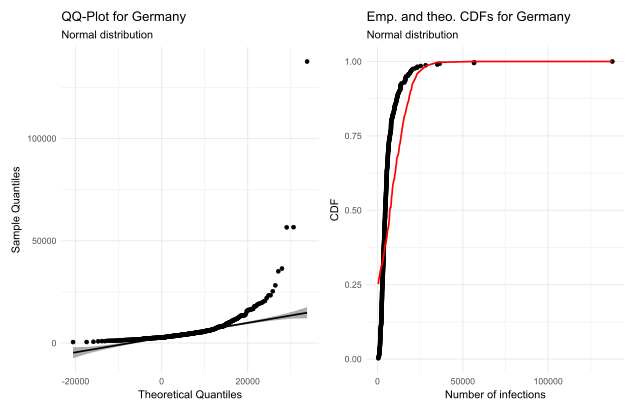
\includegraphics[width = 0.8\textwidth]{fit_normal_germany.png}
    \caption{A normal fit to the number of cases in German municipalities}
    \label{fitNormalGermany}
\end{figure}
\begin{figure}[H]
    \centering
    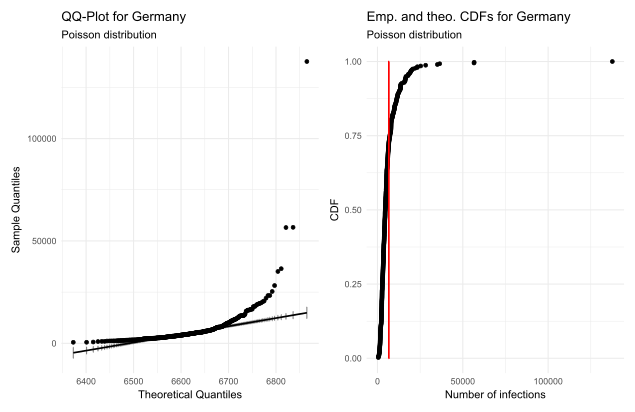
\includegraphics[width = 0.8\textwidth]{fit_poisson_germany.png}
    \caption{A Poisson fit to the number of cases in German municipalities}
    \label{fitPoissonGermany}
\end{figure}
\subsection{Distribution Fits for Norway}
\begin{figure}[H]
    \centering
    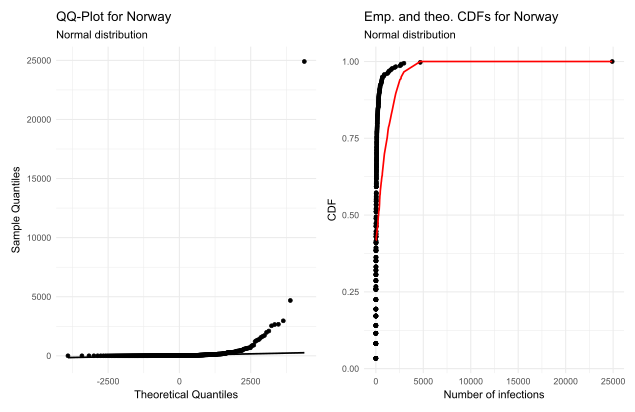
\includegraphics[width = 0.8\textwidth]{fit_normal_norway.png}
    \caption{A normal fit to the number of cases in Norwegian municipalities}
    \label{fitNormalNorway}
\end{figure}
\begin{figure}[H]
    \centering
    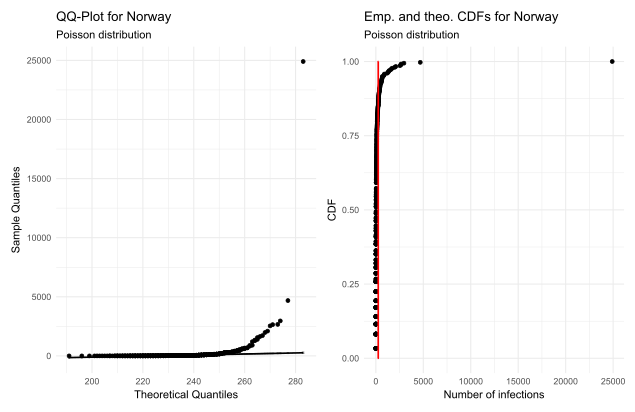
\includegraphics[width = 0.8\textwidth]{fit_poisson_norway.png}
    \caption{A Poisson fit to the number of cases in Norwegian municipalities}
    \label{fitPoissonNorway}
\end{figure}
\clearpage
\section{Choice of Hyperpriors for Germany}
\begin{figure}[H]
    \centering
    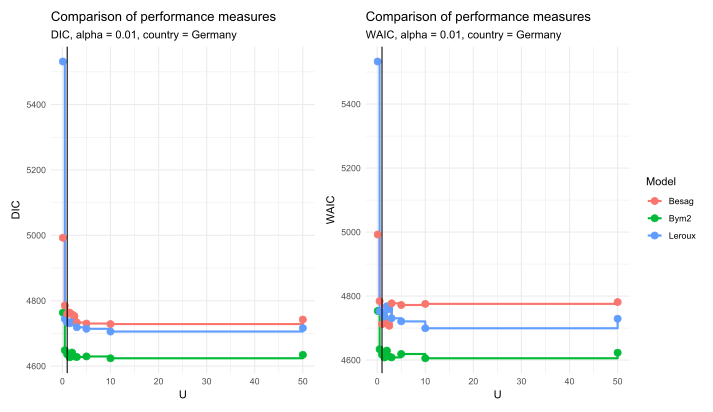
\includegraphics[width = \textwidth]{comparison_1_germany.png}
    \caption{Values of the DIC and the WAIC when changing the value for $\sigma_0$. The black line highlights the values for $\sigma_0$ = 1.}
    \label{comparison_germany_1}
\end{figure}
\begin{figure}[H]
    \centering
    \includegraphics[width = \textwidth]{mae_germany.png}
    \caption{Values of the MAE when changing the value for $\sigma_0$. The black line highlights the values for $\sigma_0$ = 1.}
    \label{comparison_germany_2}
\end{figure}
\begin{figure}[H]
    \centering
    \includegraphics[width = \textwidth]{spatial_field_germany_1.png}
    \caption{Spatial field for a Besag model and a Leroux model.}
    \label{comparison_germany_6}
\end{figure}
\begin{figure}[H]
    \centering
    \includegraphics[width = \textwidth]{spatial_field_germany_2.png}
    \caption{Spatial fields for a BYM2 model.}
    \label{comparison_germany_7}
\end{figure}
\clearpage
\section{Code Examples}
\subsection{Specifying the Different Types of Models}
\begin{lstlisting}[caption={Specifying different models in INLA.}, label={codeModels}, language=R]
# set the seed
set.seed(420)
# draw a sample
test <- sample(
    seq_len(nrow(newest_numbers)),
    size = floor(0.2 * nrow(newest_numbers))
  )
# get the number of infections for the test data
test_value <- newest_numbers$value[test]
# set the number of infections to NA in the train data
newest_numbers$value[test] <- NA
# define the link function
link <- rep(NA, nrow(newest_numbers))
link[which(is.na(newest_numbers$value))] <- 1
# for the temporal model every 5th day is taken
germany <- germany[
  germany$Date %in% seq(
    from = min(germany$Date),
    to = max(germany$Date),
    by = 5
  ),
]
# draw a sample
test_temporal <- sample(
  seq_len(nrow(germany)),
  size = floor(0.2 * nrow(germany))
)
test_value_temporal <- germany$value[test_temporal]
germany$value[test_temporal] <- NA
link_temporal <- rep(NA, nrow(germany))
link_temporal[which(is.na(germany$value))] <- 1
# define the penalised prior
prior_1 <- list(
  prec = list(
    prior = "pc.prec",
    param = c(1, 0.01)
  )
)
# create the neighbordhood matrix
nb <- poly2nb(newest_numbers)
# save the matrix
nb2INLA("maps/map.adj", nb)
g <- inla.read.graph(filename = "maps/map.adj")
# define the C matrix for the Leroux model
Q <- Diagonal(x = sapply(nb, length))
for (i in 2:nrow(newest_numbers)) {
  Q[i - 1, i] <- -1
  Q[i, i - 1] <- -1
}

C <- Diagonal(x = 1, n = nrow(newest_numbers)) - Q
# formula for the model without the spatial component
formula_1 <- value ~
  pop_dens + urb_dens + sex + trade_tax + SPD + Gruene + FDP +
  die_linke + clinic + place_of_worship + nursing_home +
  aerodrome + platform + office + marketplace + higher_education
# formula for the besag model
formula_2 <- value ~
  pop_dens + urb_dens + sex + trade_tax + SPD + Gruene + FDP +
  die_linke + clinic + place_of_worship + nursing_home +
  aerodrome + platform + office + marketplace + higher_education +
  f(idarea_1, model = "besagproper", graph = g, hyper = prior_1)
# formula for the bym2 model
formula_3 <- value ~
  pop_dens + urb_dens + sex + trade_tax + SPD + Gruene + FDP +
  die_linke + clinic + place_of_worship + nursing_home +
  aerodrome + platform + office + marketplace + higher_education +
  f(
    idarea_1, model = "bym2", graph = g,
    scale.model = TRUE, hyper = prior_1
  )
# formula for the leroux model
formula_4 <- value ~
  pop_dens + urb_dens + sex + trade_tax + SPD + Gruene + FDP +
  die_linke + clinic + place_of_worship + nursing_home +
  aerodrome + platform + office + marketplace + higher_education +
  f(idarea_1, model = "generic1", Cmatrix = C, hyper = prior_1)
# formula for the temporal bym2 model
formula_5 <- value ~
  pop_dens + urb_dens + sex + trade_tax + SPD + Gruene + FDP +
  die_linke + clinic + place_of_worship + nursing_home +
  aerodrome + platform + office + marketplace + higher_education +
  f(
    idarea_1, model = "bym2", graph = g,
    scale.model = TRUE, hyper = prior_1
  ) +
  f(id_date_1, model = "rw2", hyper = prior_1)
# compute the models
# for the non-temporal models the code looks like this
res_1 <- inla(
  formula_1,
  family = "nbinomial",
  data = newest_numbers,
  E = expected_count,
  control.predictor = list(
    compute = TRUE,
    link = link
  ),
  Ntrials = newest_numbers$population,
  control.compute = list(dic = TRUE, waic = TRUE, cpo = TRUE)
)
# for the temporal models the code looks like this
res_5 <- inla(
  formula_5,
  family = "nbinomial",
  data = germany,
  E = expected_count,
  control.predictor = list(
    compute = TRUE,
    link = link_temporal
  ),
  Ntrials = germany$population,
  control.compute = list(dic = TRUE, waic = TRUE, cpo = TRUE)
)
\end{lstlisting}
\subsection{Making Predictions for the Test Data}
\begin{lstlisting}[caption={The code for making predictions in INLA.}, label={codePrediction}, language=R]
# create a vector to save the predictions to
predicted_1 <- c()
predicted_2 <- c()
# make predictions for a non-temporal model
for (i in seq_len(nrow(newest_numbers))) {
  predicted_1[i] <- inla.emarginal(
    function(x) x * newest_numbers$population[i],
    res_1$marginals.fitted.values[[i]]
  )
}
# calculate the mae
mean(abs(predicted_1[test] - test_value)),
# make predictions for a temporal model
for (i in seq_len(nrow(germany))) {
  predicted_2[i] <- inla.emarginal(
    function(x) x * germany$population[i],
    res_5$marginals.fitted.values[[i]]
  )
}
# calculate the mae
mean(abs(predicted_2[test_temporal] - test_value_temporal)),
\end{lstlisting}
\subsection{Calculating the Posterior Mean}
\begin{lstlisting}[caption={Calculating the posterior mean of a coefficent.}, label={codePosteriorMean}, language=R]
inla.emarginal(
      exp,
      res_1$marginals.fixed$`(Intercept)`
)
\end{lstlisting}
\subsection{Calculating a Credibility Interval}
\begin{lstlisting}[caption={Extracting the credibility interval for a coefficient}, label={codeCredibility}, language=R]
inla.qmarginal(
      c(0.025, 0.975),
      inla.tmarginal(
        exp,
        res_1$marginals.fixed$`(Intercept)`
      )
)
\end{lstlisting}
\subsection{Calculating the Temporal Trend}
\begin{lstlisting}[caption={Calculating the Temporal Trend of a Model}, label={codeTemporal}, language=R]
temporal_car <- lapply(
  res_5$marginals.random$id_date_1,
  function(x) {
    marg <- inla.tmarginal(
      function(y) exp(y),
      x
    )
    inla.emarginal(mean, marg)
  }
)
\end{lstlisting}
\clearpage